\documentclass[]{article}
\usepackage{lmodern}
\usepackage{amssymb,amsmath}
\usepackage{ifxetex,ifluatex}
\usepackage{fixltx2e} % provides \textsubscript
\ifnum 0\ifxetex 1\fi\ifluatex 1\fi=0 % if pdftex
  \usepackage[T1]{fontenc}
  \usepackage[utf8]{inputenc}
\else % if luatex or xelatex
  \ifxetex
    \usepackage{mathspec}
  \else
    \usepackage{fontspec}
  \fi
  \defaultfontfeatures{Ligatures=TeX,Scale=MatchLowercase}
\fi
% use upquote if available, for straight quotes in verbatim environments
\IfFileExists{upquote.sty}{\usepackage{upquote}}{}
% use microtype if available
\IfFileExists{microtype.sty}{%
\usepackage{microtype}
\UseMicrotypeSet[protrusion]{basicmath} % disable protrusion for tt fonts
}{}
\usepackage[margin=1in]{geometry}
\usepackage{hyperref}
\hypersetup{unicode=true,
            pdftitle={Section\_1B\_worksheet},
            pdfauthor={Brie Diaz},
            pdfborder={0 0 0},
            breaklinks=true}
\urlstyle{same}  % don't use monospace font for urls
\usepackage{color}
\usepackage{fancyvrb}
\newcommand{\VerbBar}{|}
\newcommand{\VERB}{\Verb[commandchars=\\\{\}]}
\DefineVerbatimEnvironment{Highlighting}{Verbatim}{commandchars=\\\{\}}
% Add ',fontsize=\small' for more characters per line
\usepackage{framed}
\definecolor{shadecolor}{RGB}{248,248,248}
\newenvironment{Shaded}{\begin{snugshade}}{\end{snugshade}}
\newcommand{\KeywordTok}[1]{\textcolor[rgb]{0.13,0.29,0.53}{\textbf{#1}}}
\newcommand{\DataTypeTok}[1]{\textcolor[rgb]{0.13,0.29,0.53}{#1}}
\newcommand{\DecValTok}[1]{\textcolor[rgb]{0.00,0.00,0.81}{#1}}
\newcommand{\BaseNTok}[1]{\textcolor[rgb]{0.00,0.00,0.81}{#1}}
\newcommand{\FloatTok}[1]{\textcolor[rgb]{0.00,0.00,0.81}{#1}}
\newcommand{\ConstantTok}[1]{\textcolor[rgb]{0.00,0.00,0.00}{#1}}
\newcommand{\CharTok}[1]{\textcolor[rgb]{0.31,0.60,0.02}{#1}}
\newcommand{\SpecialCharTok}[1]{\textcolor[rgb]{0.00,0.00,0.00}{#1}}
\newcommand{\StringTok}[1]{\textcolor[rgb]{0.31,0.60,0.02}{#1}}
\newcommand{\VerbatimStringTok}[1]{\textcolor[rgb]{0.31,0.60,0.02}{#1}}
\newcommand{\SpecialStringTok}[1]{\textcolor[rgb]{0.31,0.60,0.02}{#1}}
\newcommand{\ImportTok}[1]{#1}
\newcommand{\CommentTok}[1]{\textcolor[rgb]{0.56,0.35,0.01}{\textit{#1}}}
\newcommand{\DocumentationTok}[1]{\textcolor[rgb]{0.56,0.35,0.01}{\textbf{\textit{#1}}}}
\newcommand{\AnnotationTok}[1]{\textcolor[rgb]{0.56,0.35,0.01}{\textbf{\textit{#1}}}}
\newcommand{\CommentVarTok}[1]{\textcolor[rgb]{0.56,0.35,0.01}{\textbf{\textit{#1}}}}
\newcommand{\OtherTok}[1]{\textcolor[rgb]{0.56,0.35,0.01}{#1}}
\newcommand{\FunctionTok}[1]{\textcolor[rgb]{0.00,0.00,0.00}{#1}}
\newcommand{\VariableTok}[1]{\textcolor[rgb]{0.00,0.00,0.00}{#1}}
\newcommand{\ControlFlowTok}[1]{\textcolor[rgb]{0.13,0.29,0.53}{\textbf{#1}}}
\newcommand{\OperatorTok}[1]{\textcolor[rgb]{0.81,0.36,0.00}{\textbf{#1}}}
\newcommand{\BuiltInTok}[1]{#1}
\newcommand{\ExtensionTok}[1]{#1}
\newcommand{\PreprocessorTok}[1]{\textcolor[rgb]{0.56,0.35,0.01}{\textit{#1}}}
\newcommand{\AttributeTok}[1]{\textcolor[rgb]{0.77,0.63,0.00}{#1}}
\newcommand{\RegionMarkerTok}[1]{#1}
\newcommand{\InformationTok}[1]{\textcolor[rgb]{0.56,0.35,0.01}{\textbf{\textit{#1}}}}
\newcommand{\WarningTok}[1]{\textcolor[rgb]{0.56,0.35,0.01}{\textbf{\textit{#1}}}}
\newcommand{\AlertTok}[1]{\textcolor[rgb]{0.94,0.16,0.16}{#1}}
\newcommand{\ErrorTok}[1]{\textcolor[rgb]{0.64,0.00,0.00}{\textbf{#1}}}
\newcommand{\NormalTok}[1]{#1}
\usepackage{graphicx,grffile}
\makeatletter
\def\maxwidth{\ifdim\Gin@nat@width>\linewidth\linewidth\else\Gin@nat@width\fi}
\def\maxheight{\ifdim\Gin@nat@height>\textheight\textheight\else\Gin@nat@height\fi}
\makeatother
% Scale images if necessary, so that they will not overflow the page
% margins by default, and it is still possible to overwrite the defaults
% using explicit options in \includegraphics[width, height, ...]{}
\setkeys{Gin}{width=\maxwidth,height=\maxheight,keepaspectratio}
\IfFileExists{parskip.sty}{%
\usepackage{parskip}
}{% else
\setlength{\parindent}{0pt}
\setlength{\parskip}{6pt plus 2pt minus 1pt}
}
\setlength{\emergencystretch}{3em}  % prevent overfull lines
\providecommand{\tightlist}{%
  \setlength{\itemsep}{0pt}\setlength{\parskip}{0pt}}
\setcounter{secnumdepth}{0}
% Redefines (sub)paragraphs to behave more like sections
\ifx\paragraph\undefined\else
\let\oldparagraph\paragraph
\renewcommand{\paragraph}[1]{\oldparagraph{#1}\mbox{}}
\fi
\ifx\subparagraph\undefined\else
\let\oldsubparagraph\subparagraph
\renewcommand{\subparagraph}[1]{\oldsubparagraph{#1}\mbox{}}
\fi

%%% Use protect on footnotes to avoid problems with footnotes in titles
\let\rmarkdownfootnote\footnote%
\def\footnote{\protect\rmarkdownfootnote}

%%% Change title format to be more compact
\usepackage{titling}

% Create subtitle command for use in maketitle
\providecommand{\subtitle}[1]{
  \posttitle{
    \begin{center}\large#1\end{center}
    }
}

\setlength{\droptitle}{-2em}

  \title{Section\_1B\_worksheet}
    \pretitle{\vspace{\droptitle}\centering\huge}
  \posttitle{\par}
    \author{Brie Diaz}
    \preauthor{\centering\large\emph}
  \postauthor{\par}
      \predate{\centering\large\emph}
  \postdate{\par}
    \date{4/19/2019}


\begin{document}
\maketitle

\begin{Shaded}
\begin{Highlighting}[]
\CommentTok{#install.packages("bio3d")}
\end{Highlighting}
\end{Shaded}

\subsection{Improve the analysis code}\label{improve-the-analysis-code}

\begin{Shaded}
\begin{Highlighting}[]
\KeywordTok{library}\NormalTok{(bio3d)}
\NormalTok{s1 <-}\StringTok{ }\KeywordTok{read.pdb}\NormalTok{(}\StringTok{"4AKE"}\NormalTok{) }\CommentTok{# kinase with drug}
\end{Highlighting}
\end{Shaded}

\begin{verbatim}
##   Note: Accessing on-line PDB file
\end{verbatim}

\begin{Shaded}
\begin{Highlighting}[]
\NormalTok{s2 <-}\StringTok{ }\KeywordTok{read.pdb}\NormalTok{(}\StringTok{"1AKE"}\NormalTok{) }\CommentTok{# kinase no drug}
\end{Highlighting}
\end{Shaded}

\begin{verbatim}
##   Note: Accessing on-line PDB file
##    PDB has ALT records, taking A only, rm.alt=TRUE
\end{verbatim}

\begin{Shaded}
\begin{Highlighting}[]
\NormalTok{s3 <-}\StringTok{ }\KeywordTok{read.pdb}\NormalTok{(}\StringTok{"1E4Y"}\NormalTok{) }\CommentTok{# kinase with drug}
\end{Highlighting}
\end{Shaded}

\begin{verbatim}
##   Note: Accessing on-line PDB file
\end{verbatim}

\begin{Shaded}
\begin{Highlighting}[]
\NormalTok{s1.chainA <-}\StringTok{ }\KeywordTok{trim.pdb}\NormalTok{(s1, }\DataTypeTok{chain=}\StringTok{"A"}\NormalTok{, }\DataTypeTok{elety=}\StringTok{"CA"}\NormalTok{)}
\NormalTok{s2.chainA <-}\StringTok{ }\KeywordTok{trim.pdb}\NormalTok{(s2, }\DataTypeTok{chain=}\StringTok{"A"}\NormalTok{, }\DataTypeTok{elety=}\StringTok{"CA"}\NormalTok{)}
\NormalTok{s3.chainA <-}\StringTok{ }\KeywordTok{trim.pdb}\NormalTok{(s3, }\DataTypeTok{chain=}\StringTok{"A"}\NormalTok{, }\DataTypeTok{elety=}\StringTok{"CA"}\NormalTok{)}
\NormalTok{s1.b <-}\StringTok{ }\NormalTok{s1.chainA}\OperatorTok{$}\NormalTok{atom}\OperatorTok{$}\NormalTok{b}
\NormalTok{s2.b <-}\StringTok{ }\NormalTok{s2.chainA}\OperatorTok{$}\NormalTok{atom}\OperatorTok{$}\NormalTok{b}
\NormalTok{s3.b <-}\StringTok{ }\NormalTok{s3.chainA}\OperatorTok{$}\NormalTok{atom}\OperatorTok{$}\NormalTok{b}
\KeywordTok{plotb3}\NormalTok{(s1.b, }\DataTypeTok{sse=}\NormalTok{s1.chainA, }\DataTypeTok{typ=}\StringTok{"l"}\NormalTok{, }\DataTypeTok{ylab=}\StringTok{"Bfactor"}\NormalTok{)}
\end{Highlighting}
\end{Shaded}

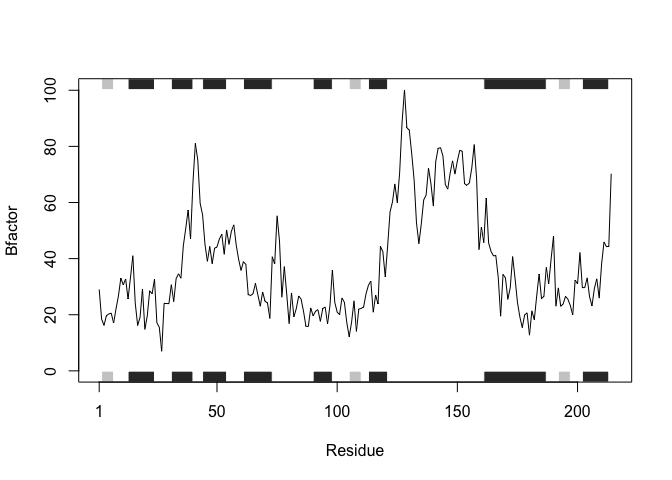
\includegraphics{class06_worksheet_files/figure-latex/unnamed-chunk-2-1.pdf}

\begin{Shaded}
\begin{Highlighting}[]
\KeywordTok{plotb3}\NormalTok{(s2.b, }\DataTypeTok{sse=}\NormalTok{s2.chainA, }\DataTypeTok{typ=}\StringTok{"l"}\NormalTok{, }\DataTypeTok{ylab=}\StringTok{"Bfactor"}\NormalTok{)}
\end{Highlighting}
\end{Shaded}

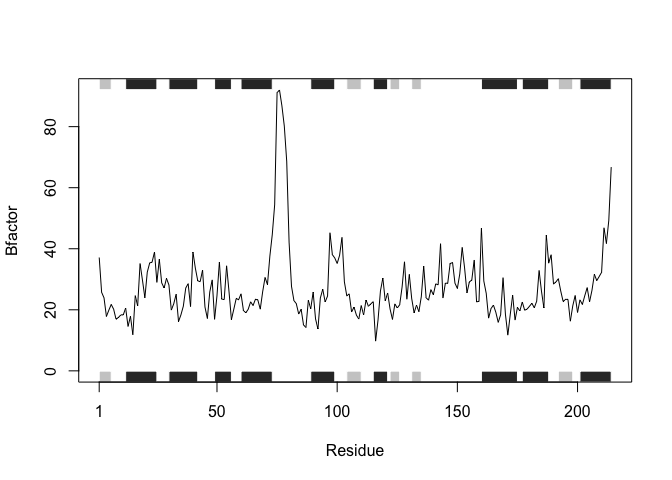
\includegraphics{class06_worksheet_files/figure-latex/unnamed-chunk-2-2.pdf}

\begin{Shaded}
\begin{Highlighting}[]
\KeywordTok{plotb3}\NormalTok{(s3.b, }\DataTypeTok{sse=}\NormalTok{s3.chainA, }\DataTypeTok{typ=}\StringTok{"l"}\NormalTok{, }\DataTypeTok{ylab=}\StringTok{"Bfactor"}\NormalTok{)}
\end{Highlighting}
\end{Shaded}

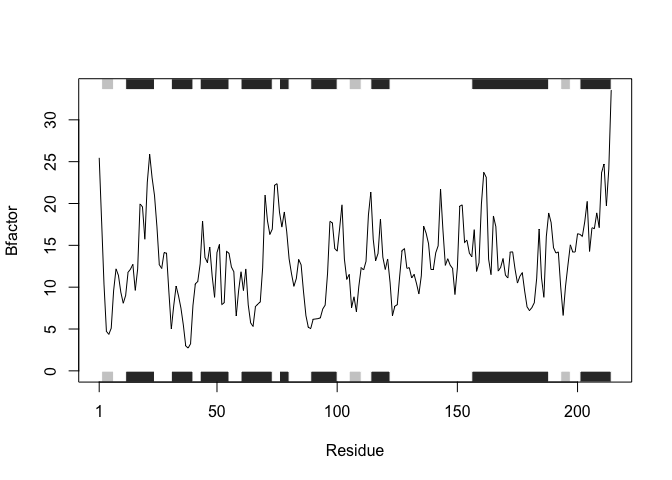
\includegraphics{class06_worksheet_files/figure-latex/unnamed-chunk-2-3.pdf}

\subsection{Q1 What type of object is returned from the read.pdb()
function?}\label{q1-what-type-of-object-is-returned-from-the-read.pdb-function}

\begin{Shaded}
\begin{Highlighting}[]
\KeywordTok{is.list}\NormalTok{(s1)}
\end{Highlighting}
\end{Shaded}

\begin{verbatim}
## [1] TRUE
\end{verbatim}

\begin{itemize}
\tightlist
\item
  the read.pdb() function reads a PDB file and returns a list
\end{itemize}

\subsection{Q2 What does the trim.pbd() function
do?}\label{q2-what-does-the-trim.pbd-function-do}

\begin{Shaded}
\begin{Highlighting}[]
\NormalTok{?trim.pdb}
\end{Highlighting}
\end{Shaded}

\begin{itemize}
\tightlist
\item
  Trims a PBD object to a subset of atoms; description: produces a new
  smaller PDB object, containing a subset of atoms, from a given larger
  PDB object
\end{itemize}

\subsection{Q3 What input parameter would turn off the marginal black
and gray rectangles in the plots and what do they represent in this
case?}\label{q3-what-input-parameter-would-turn-off-the-marginal-black-and-gray-rectangles-in-the-plots-and-what-do-they-represent-in-this-case}

\begin{itemize}
\tightlist
\item
  remove sse or set to FALSE; also, you could set both top = FALSE and
  bot = FALSE
\end{itemize}

\begin{Shaded}
\begin{Highlighting}[]
\NormalTok{?plot.bio3d}
\end{Highlighting}
\end{Shaded}

plotb3 draws a standard scatter plot with optional secondary structure
in the marginal regions

\subsection{Q5 Which proteins are more similar to each other in their
B-factor
trends}\label{q5-which-proteins-are-more-similar-to-each-other-in-their-b-factor-trends}

\begin{Shaded}
\begin{Highlighting}[]
\NormalTok{hc <-}\StringTok{ }\KeywordTok{hclust}\NormalTok{(}\KeywordTok{dist}\NormalTok{(}\KeywordTok{rbind}\NormalTok{(s1.b, s2.b, s3.b)))}
\KeywordTok{plot}\NormalTok{(hc)}
\end{Highlighting}
\end{Shaded}

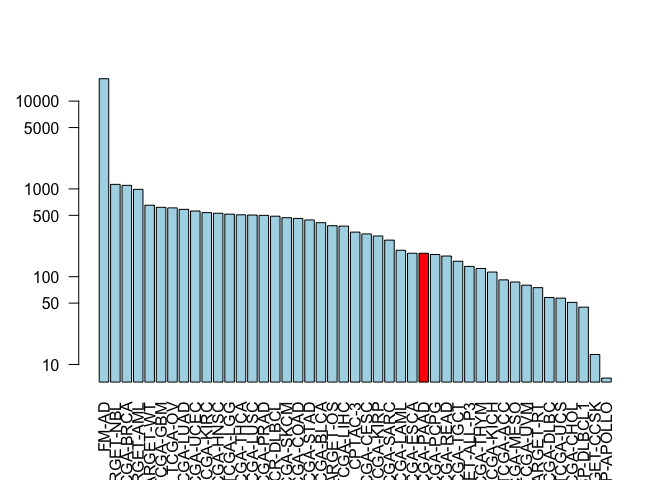
\includegraphics{class06_worksheet_files/figure-latex/unnamed-chunk-6-1.pdf}

\begin{itemize}
\tightlist
\item
  Proteins 1AKE and 1E4Y (represented by s2.b and s3.b, respectively)
  are more similar to each other
\end{itemize}

\subsection{Q6 How would you generalize the original code above to work
with any set of input protein
structures?}\label{q6-how-would-you-generalize-the-original-code-above-to-work-with-any-set-of-input-protein-structures}

\subsubsection{Don't ever start like this: copy and paste each line of
function}\label{dont-ever-start-like-this-copy-and-paste-each-line-of-function}

makeplot \textless{}- function(x) \{ s1 \textless{}- read.pdb(x) \#
kinase with drug s1.chainA \textless{}- trim.pdb(s1, chain=``A'',
elety=``CA'') s1.b \textless{}- s1.chainA\(atom\)b plotb3(s1.b,
sse=s1.chainA, typ=``l'', ylab=``Bfactor'') \}

\subsubsection{instead, make small working snippets of
code}\label{instead-make-small-working-snippets-of-code}

First, access the proteins sequence from PDP and save as ``pseq''

\begin{Shaded}
\begin{Highlighting}[]
\NormalTok{x <-}\StringTok{ "4AKE"}
\NormalTok{pseq <-}\StringTok{ }\KeywordTok{read.pdb}\NormalTok{(x)}
\end{Highlighting}
\end{Shaded}

\begin{verbatim}
##   Note: Accessing on-line PDB file
\end{verbatim}

\begin{verbatim}
## Warning in get.pdb(file, path = tempdir(), verbose = FALSE): /var/folders/
## 2l/s152rlf121v7z6zp2br1y6bw0000gn/T//RtmpUrZJ9C/4AKE.pdb exists. Skipping
## download
\end{verbatim}

\begin{Shaded}
\begin{Highlighting}[]
\NormalTok{pseq}
\end{Highlighting}
\end{Shaded}

\begin{verbatim}
## 
##  Call:  read.pdb(file = x)
## 
##    Total Models#: 1
##      Total Atoms#: 3459,  XYZs#: 10377  Chains#: 2  (values: A B)
## 
##      Protein Atoms#: 3312  (residues/Calpha atoms#: 428)
##      Nucleic acid Atoms#: 0  (residues/phosphate atoms#: 0)
## 
##      Non-protein/nucleic Atoms#: 147  (residues: 147)
##      Non-protein/nucleic resid values: [ HOH (147) ]
## 
##    Protein sequence:
##       MRIILLGAPGAGKGTQAQFIMEKYGIPQISTGDMLRAAVKSGSELGKQAKDIMDAGKLVT
##       DELVIALVKERIAQEDCRNGFLLDGFPRTIPQADAMKEAGINVDYVLEFDVPDELIVDRI
##       VGRRVHAPSGRVYHVKFNPPKVEGKDDVTGEELTTRKDDQEETVRKRLVEYHQMTAPLIG
##       YYSKEAEAGNTKYAKVDGTKPVAEVRADLEKILGMRIILLGAPGA...<cut>...KILG
## 
## + attr: atom, xyz, seqres, helix, sheet,
##         calpha, remark, call
\end{verbatim}

Next, trim protein sequence so that it includes only chain A of the
protein.

\begin{Shaded}
\begin{Highlighting}[]
\NormalTok{pseq.chainA <-}\StringTok{ }\KeywordTok{trim.pdb}\NormalTok{(pseq, }\DataTypeTok{chain=}\StringTok{"A"}\NormalTok{, }\DataTypeTok{elety=}\StringTok{"CA"}\NormalTok{)}
\NormalTok{pseq.chainA}
\end{Highlighting}
\end{Shaded}

\begin{verbatim}
## 
##  Call:  trim.pdb(pdb = pseq, chain = "A", elety = "CA")
## 
##    Total Models#: 1
##      Total Atoms#: 214,  XYZs#: 642  Chains#: 1  (values: A)
## 
##      Protein Atoms#: 214  (residues/Calpha atoms#: 214)
##      Nucleic acid Atoms#: 0  (residues/phosphate atoms#: 0)
## 
##      Non-protein/nucleic Atoms#: 0  (residues: 0)
##      Non-protein/nucleic resid values: [ none ]
## 
##    Protein sequence:
##       MRIILLGAPGAGKGTQAQFIMEKYGIPQISTGDMLRAAVKSGSELGKQAKDIMDAGKLVT
##       DELVIALVKERIAQEDCRNGFLLDGFPRTIPQADAMKEAGINVDYVLEFDVPDELIVDRI
##       VGRRVHAPSGRVYHVKFNPPKVEGKDDVTGEELTTRKDDQEETVRKRLVEYHQMTAPLIG
##       YYSKEAEAGNTKYAKVDGTKPVAEVRADLEKILG
## 
## + attr: atom, helix, sheet, seqres, xyz,
##         calpha, call
\end{verbatim}

Next, access the Temperature factor, represented by the ``b'' vector
within the ``atom'' data frame for this trimmed sequence

\begin{Shaded}
\begin{Highlighting}[]
\NormalTok{pseq.chainA <-}\StringTok{ }\KeywordTok{trim.pdb}\NormalTok{(pseq, }\DataTypeTok{chain=}\StringTok{"A"}\NormalTok{, }\DataTypeTok{elety=}\StringTok{"CA"}\NormalTok{)}
\NormalTok{pseq.b <-}\StringTok{ }\NormalTok{pseq.chainA}\OperatorTok{$}\NormalTok{atom}\OperatorTok{$}\NormalTok{b}
\end{Highlighting}
\end{Shaded}

Make a line plot of the Temperature Factor data with the y-axis labeled
``Bfactor''

\begin{Shaded}
\begin{Highlighting}[]
\NormalTok{pseq.chainA <-}\StringTok{ }\KeywordTok{trim.pdb}\NormalTok{(pseq, }\DataTypeTok{chain=}\StringTok{"A"}\NormalTok{, }\DataTypeTok{elety=}\StringTok{"CA"}\NormalTok{)}
\NormalTok{pseq.b <-}\StringTok{ }\NormalTok{pseq.chainA}\OperatorTok{$}\NormalTok{atom}\OperatorTok{$}\NormalTok{b}
\KeywordTok{plotb3}\NormalTok{(pseq.b, }\DataTypeTok{sse=}\NormalTok{pseq.chainA, }\DataTypeTok{type =} \StringTok{"l"}\NormalTok{, }\DataTypeTok{ylab=}\StringTok{"Bfactor"}\NormalTok{)}
\end{Highlighting}
\end{Shaded}

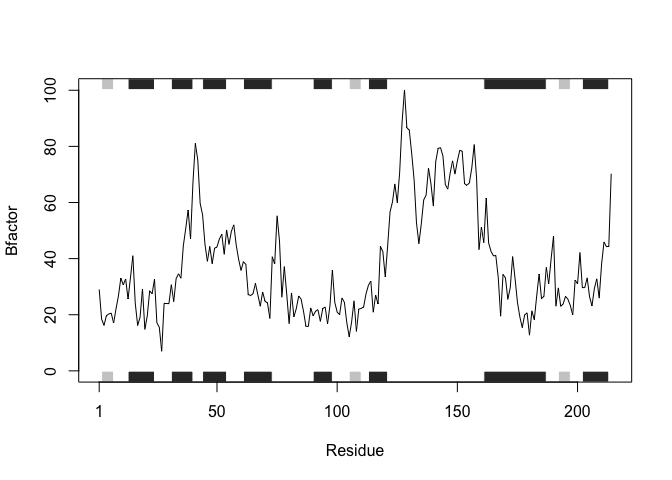
\includegraphics{class06_worksheet_files/figure-latex/unnamed-chunk-10-1.pdf}

Finally, turn overall working snippets into a function!

\begin{itemize}
\item
  The input(x) is a name of a protein sequence in PDB; simply set x =
  ``\emph{name\_of\_PDB\_seq}'' in the function itself
\item
  the function will:
\end{itemize}

\begin{enumerate}
\def\labelenumi{\arabic{enumi}.}
\tightlist
\item
  read the PDF sequence you assign to it
\item
  trim your protein sequence to include chain A alpha carbons; creates a
  new PDB object based on a selection of atoms
\item
  access the B factor (Temperature Factor) for all atoms in the trimmed
  protein sequence
\item
  produce a line plot of Residue vs.~B Factor --\textgreater{} this is
  the overall output of the function!
\end{enumerate}

\begin{Shaded}
\begin{Highlighting}[]
\NormalTok{makeplot <-}\StringTok{ }\ControlFlowTok{function}\NormalTok{(x) \{}
\NormalTok{  pseq <-}\StringTok{ }\KeywordTok{read.pdb}\NormalTok{(x)}
\NormalTok{  pseq.chainA <-}\StringTok{ }\KeywordTok{trim.pdb}\NormalTok{(pseq, }\DataTypeTok{chain=}\StringTok{"A"}\NormalTok{, }\DataTypeTok{elety=}\StringTok{"CA"}\NormalTok{)}
\NormalTok{  pseq.b <-}\StringTok{ }\NormalTok{pseq.chainA}\OperatorTok{$}\NormalTok{atom}\OperatorTok{$}\NormalTok{b}
  \KeywordTok{plotb3}\NormalTok{(pseq.b, }\DataTypeTok{sse=}\NormalTok{pseq.chainA, }\DataTypeTok{type =} \StringTok{"l"}\NormalTok{, }\DataTypeTok{ylab=}\StringTok{"Bfactor"}\NormalTok{)}
\NormalTok{\}}
\end{Highlighting}
\end{Shaded}

Test out new function:

\begin{Shaded}
\begin{Highlighting}[]
\KeywordTok{makeplot}\NormalTok{(}\StringTok{"4AKE"}\NormalTok{)}
\end{Highlighting}
\end{Shaded}

\begin{verbatim}
##   Note: Accessing on-line PDB file
\end{verbatim}

\begin{verbatim}
## Warning in get.pdb(file, path = tempdir(), verbose = FALSE): /var/folders/
## 2l/s152rlf121v7z6zp2br1y6bw0000gn/T//RtmpUrZJ9C/4AKE.pdb exists. Skipping
## download
\end{verbatim}

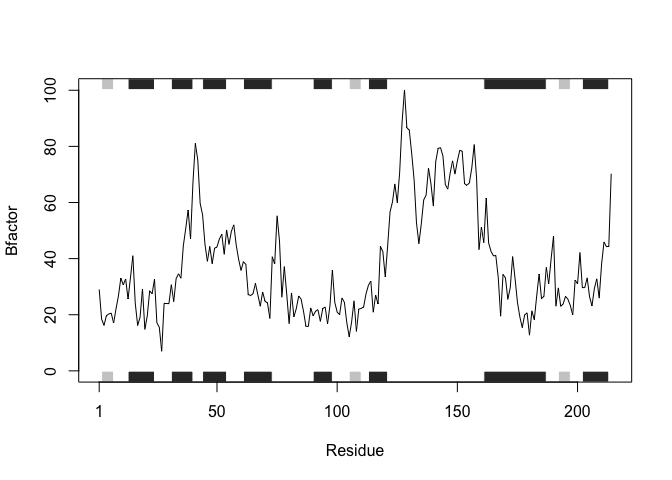
\includegraphics{class06_worksheet_files/figure-latex/unnamed-chunk-12-1.pdf}

\begin{Shaded}
\begin{Highlighting}[]
\KeywordTok{makeplot}\NormalTok{(}\StringTok{"1AKE"}\NormalTok{)}
\end{Highlighting}
\end{Shaded}

\begin{verbatim}
##   Note: Accessing on-line PDB file
\end{verbatim}

\begin{verbatim}
## Warning in get.pdb(file, path = tempdir(), verbose = FALSE): /var/folders/
## 2l/s152rlf121v7z6zp2br1y6bw0000gn/T//RtmpUrZJ9C/1AKE.pdb exists. Skipping
## download
\end{verbatim}

\begin{verbatim}
##    PDB has ALT records, taking A only, rm.alt=TRUE
\end{verbatim}

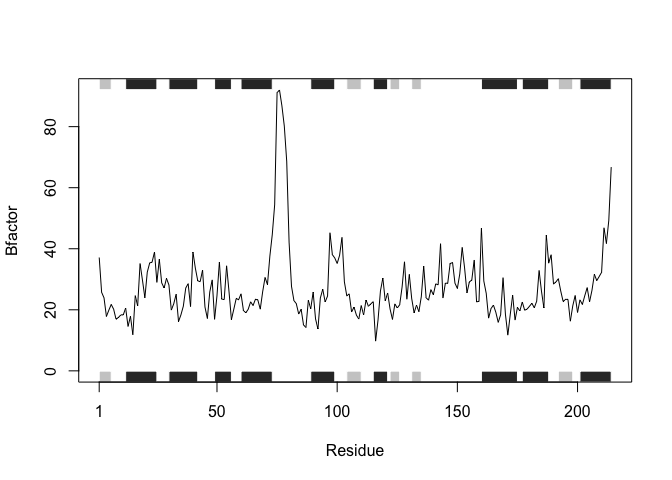
\includegraphics{class06_worksheet_files/figure-latex/unnamed-chunk-12-2.pdf}

\begin{Shaded}
\begin{Highlighting}[]
\KeywordTok{makeplot}\NormalTok{(}\StringTok{"1E4Y"}\NormalTok{)}
\end{Highlighting}
\end{Shaded}

\begin{verbatim}
##   Note: Accessing on-line PDB file
\end{verbatim}

\begin{verbatim}
## Warning in get.pdb(file, path = tempdir(), verbose = FALSE): /var/folders/
## 2l/s152rlf121v7z6zp2br1y6bw0000gn/T//RtmpUrZJ9C/1E4Y.pdb exists. Skipping
## download
\end{verbatim}

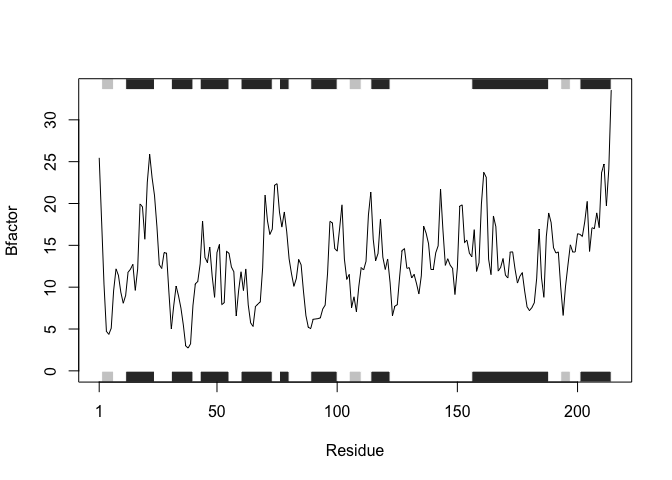
\includegraphics{class06_worksheet_files/figure-latex/unnamed-chunk-12-3.pdf}


\end{document}
